\section{Introduction}

% Tracing algorithms is ubiquitous, fundamental
Tracing algorithms on concrete examples is fundamental to teaching and learning
in CS education~\cite{Lister2004}, but drawing on blackboards and paper can be
tedious and limiting. First, these media do not afford manipulation of the
drawing, requiring the user to storyboard the behavior as a series of static
snapshots. Second, the drawing process is not recorded in a persistent format,
making it hard for students and teachers to discuss problems unless they are
co-located.
% This limitation is particularly problematic in a MOOC context, where the
% majority of students do not have direct access to teaching staff.

\begin{figure}

\begin{center}
%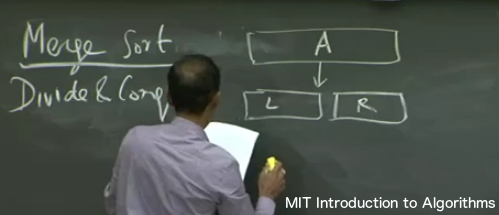
\includegraphics[width=0.55\columnwidth]{img/frontpage-6006.png}
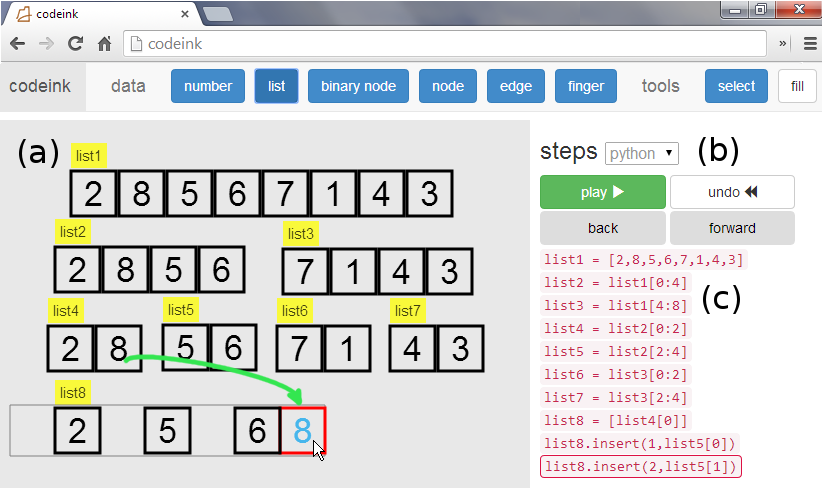
\includegraphics[width=\columnwidth]{img/frontpage-mergesort.png}
\end{center}

\caption{CodeInk is a Web-based environment that enables teachers and students
to trace algorithms on examples by direct manipulation. The user can (a) compose and
manipulate data structures, (b) step through the recorded trace, and (c) see
each step translated into a line of Python code or an English explanation.}

\label{fig:codeink-intro}
\end{figure}

We hypothesize that the ideal user interface for teaching and learning
algorithms should (a) afford direct manipulation of data structures, and (b)
record the trace in a structured format that can be disseminated and discussed.

To explore this, we built \emph{CodeInk}, a Web-based environment for tracing
algorithms by direct manipulation (DM). It includes a DM gesture set that
enables users to transform lists, trees and graphs rather than tediously draw
snapshots. When the user manipulates data structures, the trace is recorded as
interactive program steps, in Python or explanatory English. The steps provide
three main benefits: feedback on user interactions, navigation through the
trace, and a format that can be easily disseminated and analyzed as a basis for
discussion. This paper makes the following primary contributions:

\begin{comment}
\fig{fig:codeink-intro} shows how an instructor can explain the merge sort
algorithm in CodeInk by dragging an example list onto the canvas, selecting
sublists with a rectangular selection, dragging them away to create copies, then
merging elements by dragging them into a new sorted list
(\fig{fig:codeink-intro}a).
Every interaction is interpreted as a step in Python (\fig{fig:codeink-intro}c).
The trace can then be shared with students, who can navigate through it by
single-stepping or clicking on steps (\fig{fig:codeink-intro}b), and then trace
the algorithm for themselves on a new example. Their own trace can be shared
with teachers as a basis for feedback on not just the final output, but also the
process by which the list was sorted.
\end{comment}


\begin{enumerate}

\item The design of a direct manipulation (DM) gesture set for tracing algorithm
behavior on lists, trees and graphs.

\item CodeInk: an environment for tracing algorithms that implements the DM
gesture set and records traces as sharable, interactive program steps.

\item An evaluation of CodeInk's viability in a controlled study, where students
watched CodeInk-produced traces to learn an algorithm, and then used CodeInk to
trace the algorithm on a new example to solidify their understanding.

\end{enumerate}

% \pg{talk broader about future implications for this sort of technique}
\begin{comment}
While our focus is on enhancing algorithm traces in a CS education context, the
ability to directly manipulate data structures and record those interactions as
program steps may have broader applicability: for the general programmer, it may
enable better visualization and exploration of an algorithm's design. We
conclude this paper with a discussion of future work.
\end{comment}